\section{Sinusoidal as $f(t)$ with Half-Box Kernel}

Compute the convolution of a given signal \( f(t) \) with a rectangular kernel \( h(t) \), analytically. The rectangular kernel is defined as:
\[
h(t) = 
\begin{cases}
1, & \text{for } -T \leq t \leq T, \\
0, & \text{otherwise}.
\end{cases}
\]
...

\subsection{Modify the kernel to only consider the part of the kernel for \( t > 0 \). How does this affect the convolution result?}

\subsubsection{Analytic}
In this analysis, we investigate the convolution of a sinusoidal input signal
\[
f(t) = A \sin(\omega t + \phi)
\]
with a rectangular kernel that is modified as below. The modified rectangular kernel is defined as:

\[
h(t) =
\begin{cases}
1, & \text{for } 0 < t < T, \\
0, & \text{otherwise}.
\end{cases}
\]

Our goal is to derive the convolution expression \( y(t) = (f \ast h)(t) \) analytically and analyze the system’s behavior.

The convolution of \( f(t) \) and \( h(t) \) is defined as:
\[
y(t) = (f \ast h)(t) = \int_{-\infty}^{\infty} f(\tau) h(t - \tau) \, d\tau
\]

Substituting our functions:
\[
y(t) = \int_{-\infty}^{\infty} A \sin(\omega \tau + \phi) \cdot h(t - \tau) \, d\tau
\]

Since the kernel \( h(t - \tau) \) is non-zero only when \( 0  < t - \tau <  T \), we can rewrite this condition as:
\[
t - T < \tau < t
\]

Therefore, the limits of integration become:
\[
y(t) = \int_{t - T}^{t} A \sin(\omega \tau + \phi) \, d\tau
\]

Evaluating this integral:
The integral of \( \sin(\omega \tau + \phi) \) is:
\[
\int \sin(\omega \tau + \phi) \, d\tau = -\frac{1}{\omega} \cos(\omega \tau + \phi)
\]

Evaluating the integral from \( t - T \) to \( t \):
\[
y(t) = A \left[ -\frac{1}{\omega} \cos(\omega \tau + \phi) \right]_{t - T}^{t}
\]

This simplifies to:
\[
y(t) = A \left( -\frac{1}{\omega} \cos(\omega t + \phi) + \frac{1}{\omega} \cos(\omega (t - T) + \phi) \right)
\]
Using the identity for the difference of cosines:
\[
\cos A - \cos B = -2 \sin\left( \frac{A + B}{2} \right) \sin\left( \frac{A - B}{2} \right)
\]
\[
y(t) = \frac{A}{\omega} \left( -2 \sin \left( \frac{(\omega (t - T) + \phi) + (\omega t + \phi)}{2} \right) \sin \left( \frac{(\omega (t - T) + \phi) - (\omega t + \phi)}{2} \right) \right)
\]
\[
y(t) = \frac{A}{\omega} \left( -2 \sin \left( \omega t + \phi - \frac{\omega T}{2} \right) \sin \left( \frac{\omega T}{2} \right) \right)
\]
\[
\boxed{y(t) = \frac{2A \sin\left( \frac{\omega T}{2} \right)}{\omega} \sin \left( \omega( t  - \frac{T}{2}) + \phi \right)}
\]
The convolution for the modified kernel does not change the behavior of the signal, i.e., the output still remains sinusoidal.The significant differences are as follows :
\begin{itemize}
\item A $ \frac{T}{2} $ time shift towards right .

\item The scaling of amplitude is changed from $\frac{2\sin(\omega T)}{\omega}$ to $\frac{2\sin(\frac{\omega T}{2})}{\omega}$ .
\end{itemize}

\begin{figure}
    \centering
    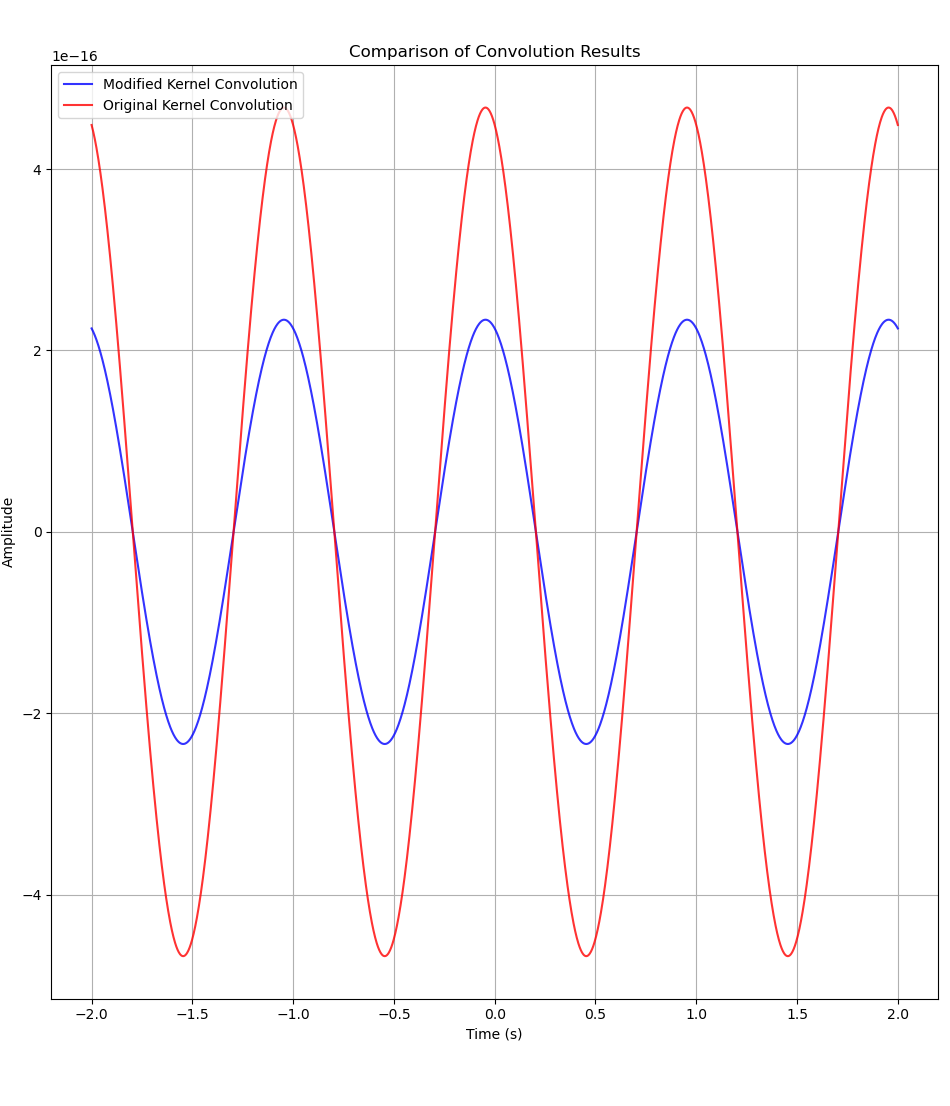
\includegraphics[width=0.5\linewidth]{codes/codes_sin_2/figs/compare.png}
    \caption{Plot of the convolutions}
    \label{fig:enter-label}
\end{figure}

\newpage

\subsection{Extended Graphical and Analytical Analysis}

\subsubsection{Effect of Amplitude \( A \)}

The first figure below demonstrates the impact of changing amplitude values on the convolution result. As seen, increasing the amplitude scales the overall magnitude of the output signal, keeping the shape unchanged.
\begin{figure}[h]
    \centering
    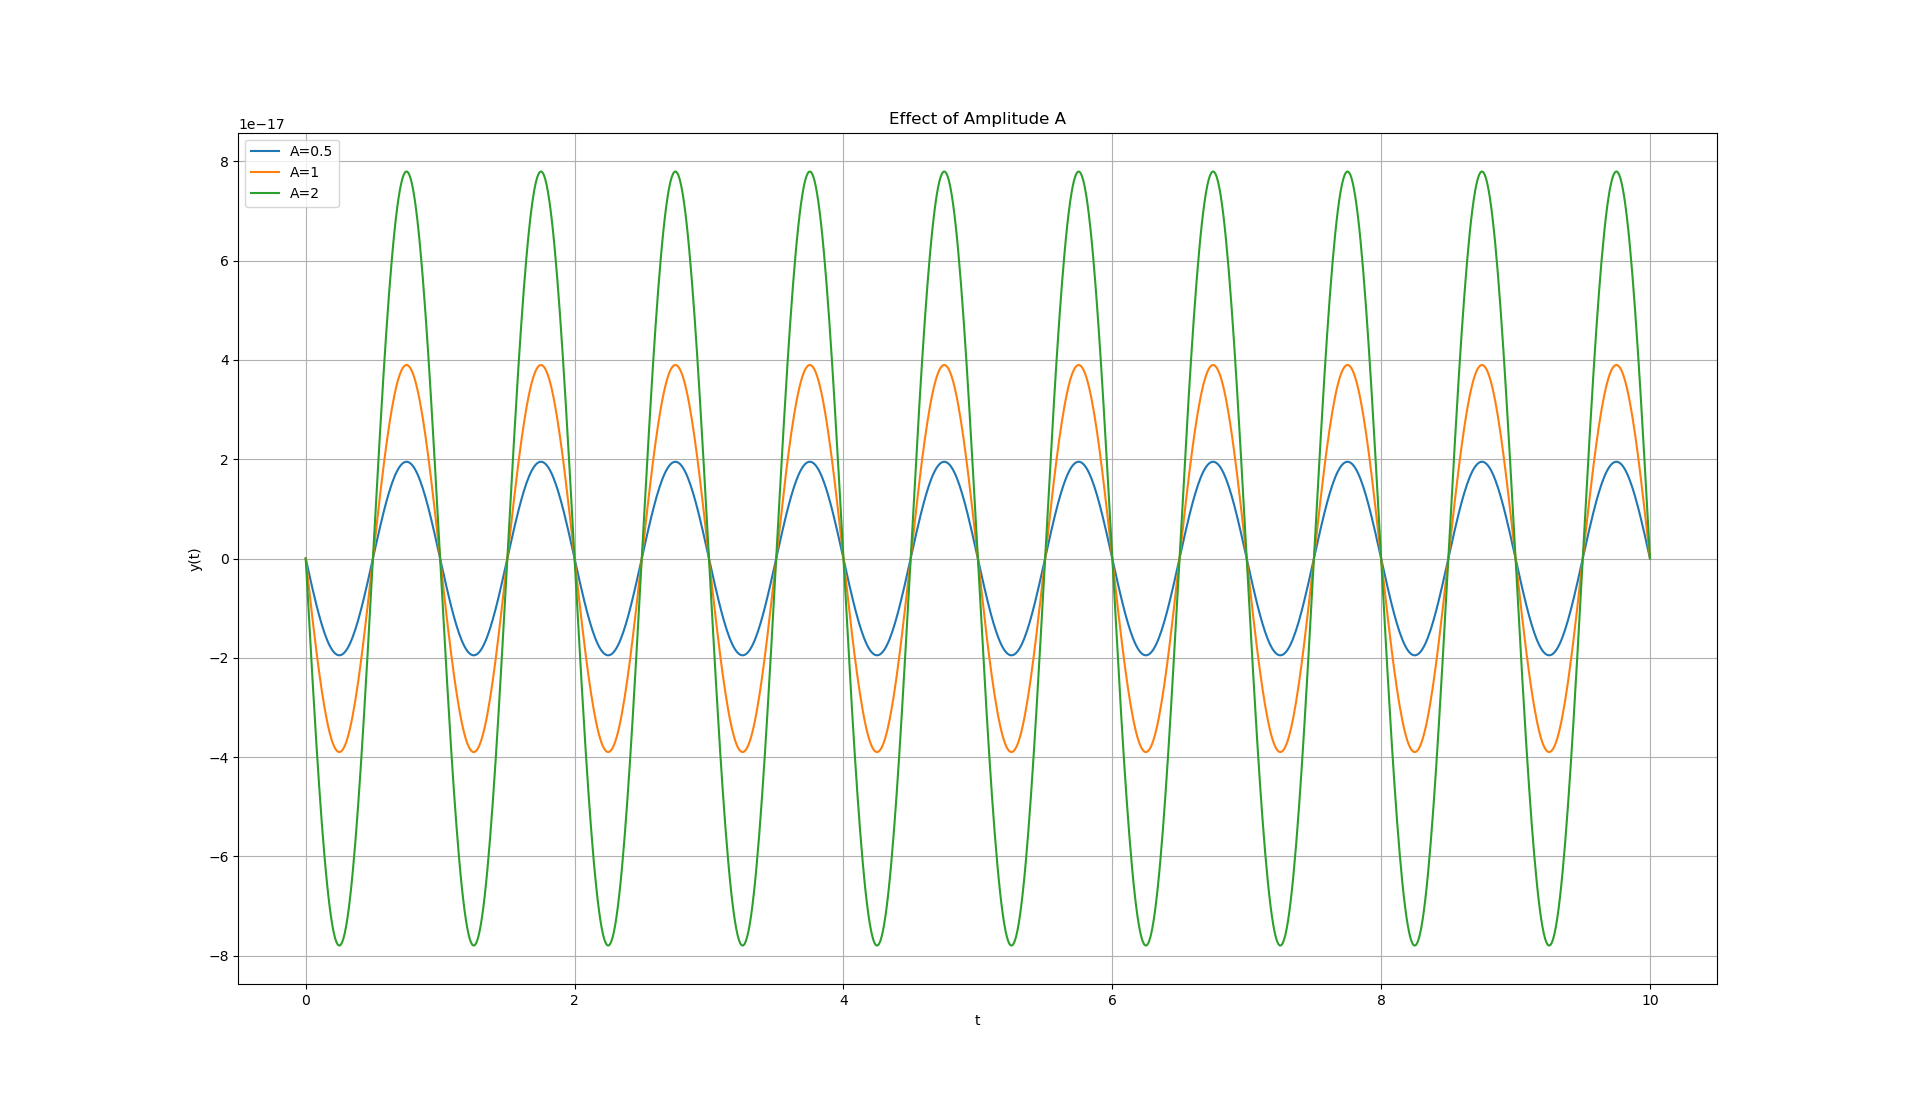
\includegraphics[width=0.8\textwidth]{codes/codes_sin_2/figs/amp.png}
    \caption{Effect of varying amplitude \( A \) on the convolution output.}
\end{figure}



\subsubsection{Effect of Angular Frequency \( \omega \)}

Changing \( \omega \) changes how rapidly the sinusoidal input oscillates. This figure shows how higher frequencies start diminishing in magnitude due to the sinc-type attenuation from the convolution.
\begin{figure}[h]
    \centering
    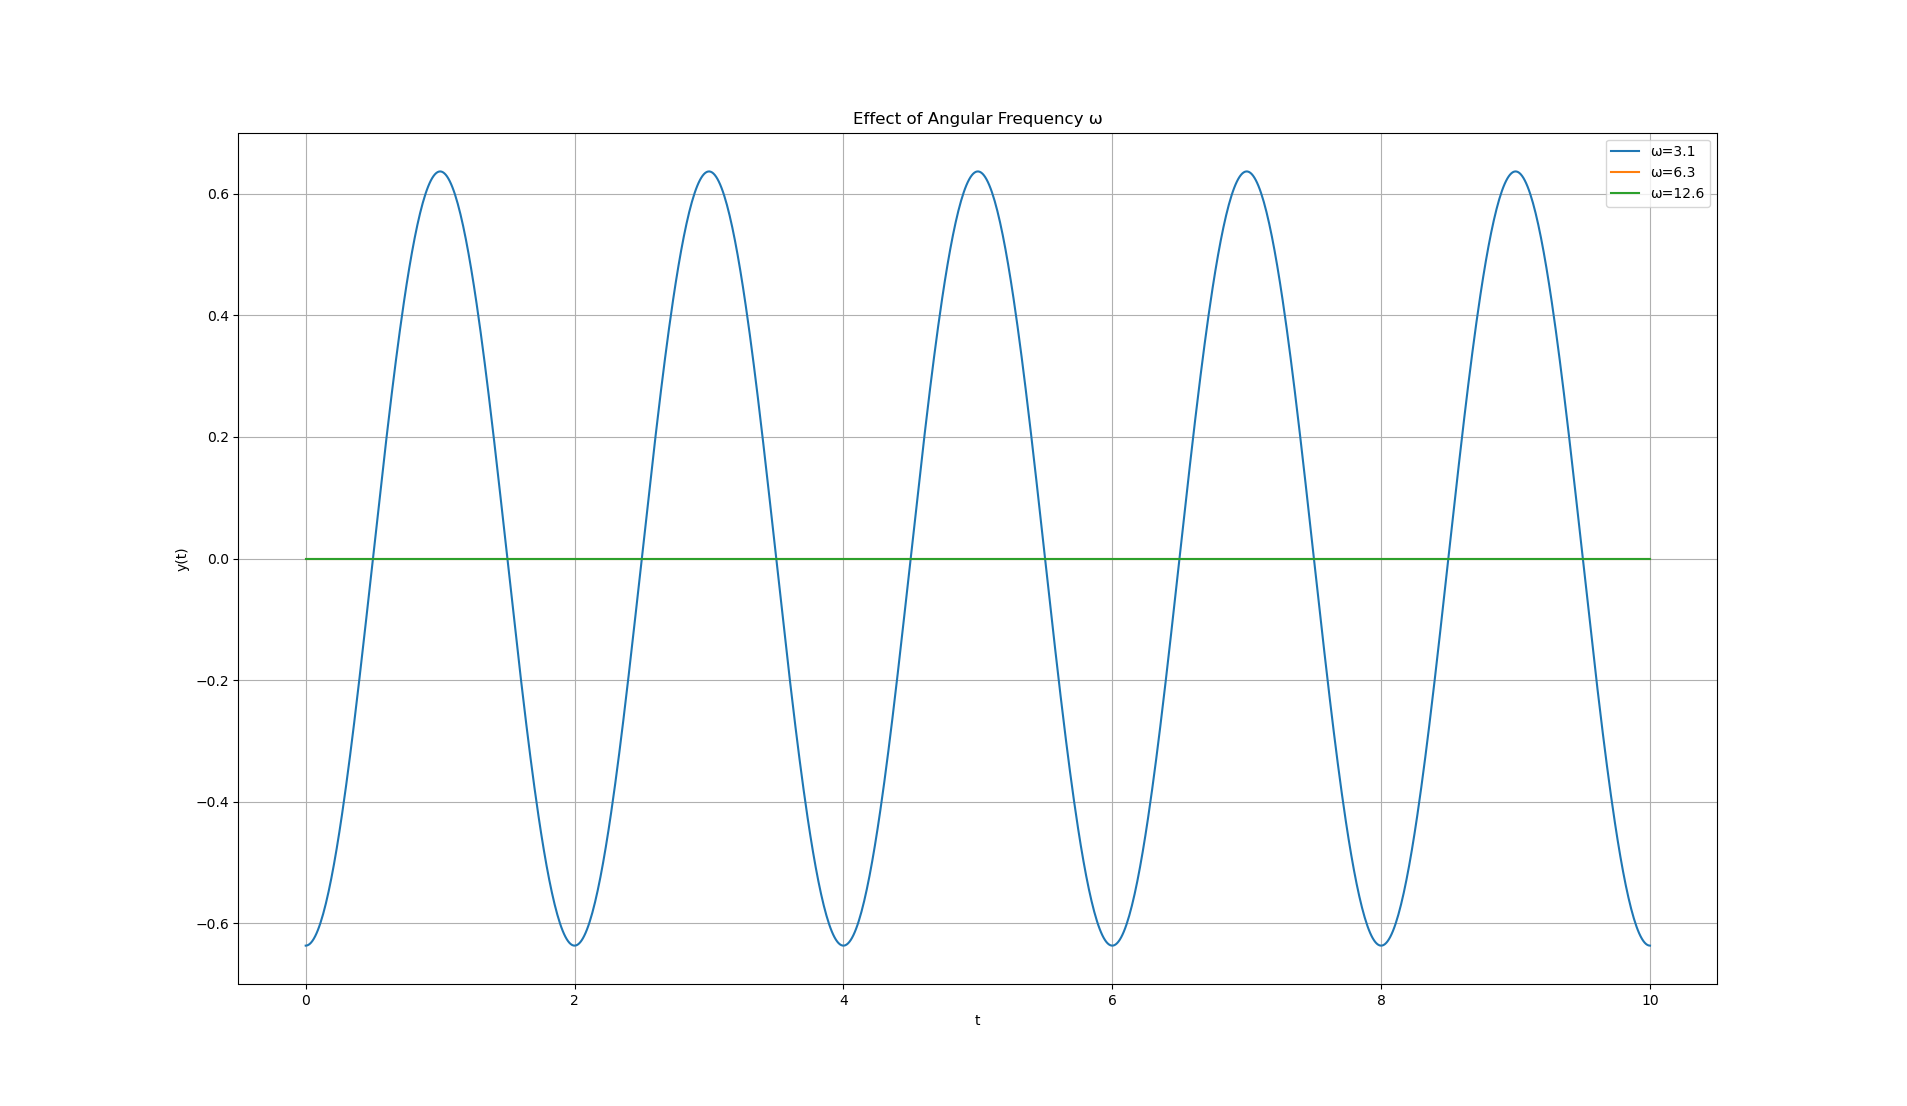
\includegraphics[width=0.8\textwidth]{codes/codes_sin_2/figs/omega.png}
    \caption{Effect of angular frequency \( \omega \) on convolution. Higher frequencies are attenuated.}
\end{figure}

\subsubsection{Effect of Pulse Width \( T \)}

This graph demonstrates how varying \( T \), the width of the rectangular kernel, influences the output. Smaller \( T \) leads to lesser averaging, preserving high-frequency content. Larger \( T \) results in more smoothing.
\begin{figure}[h]
    \centering
    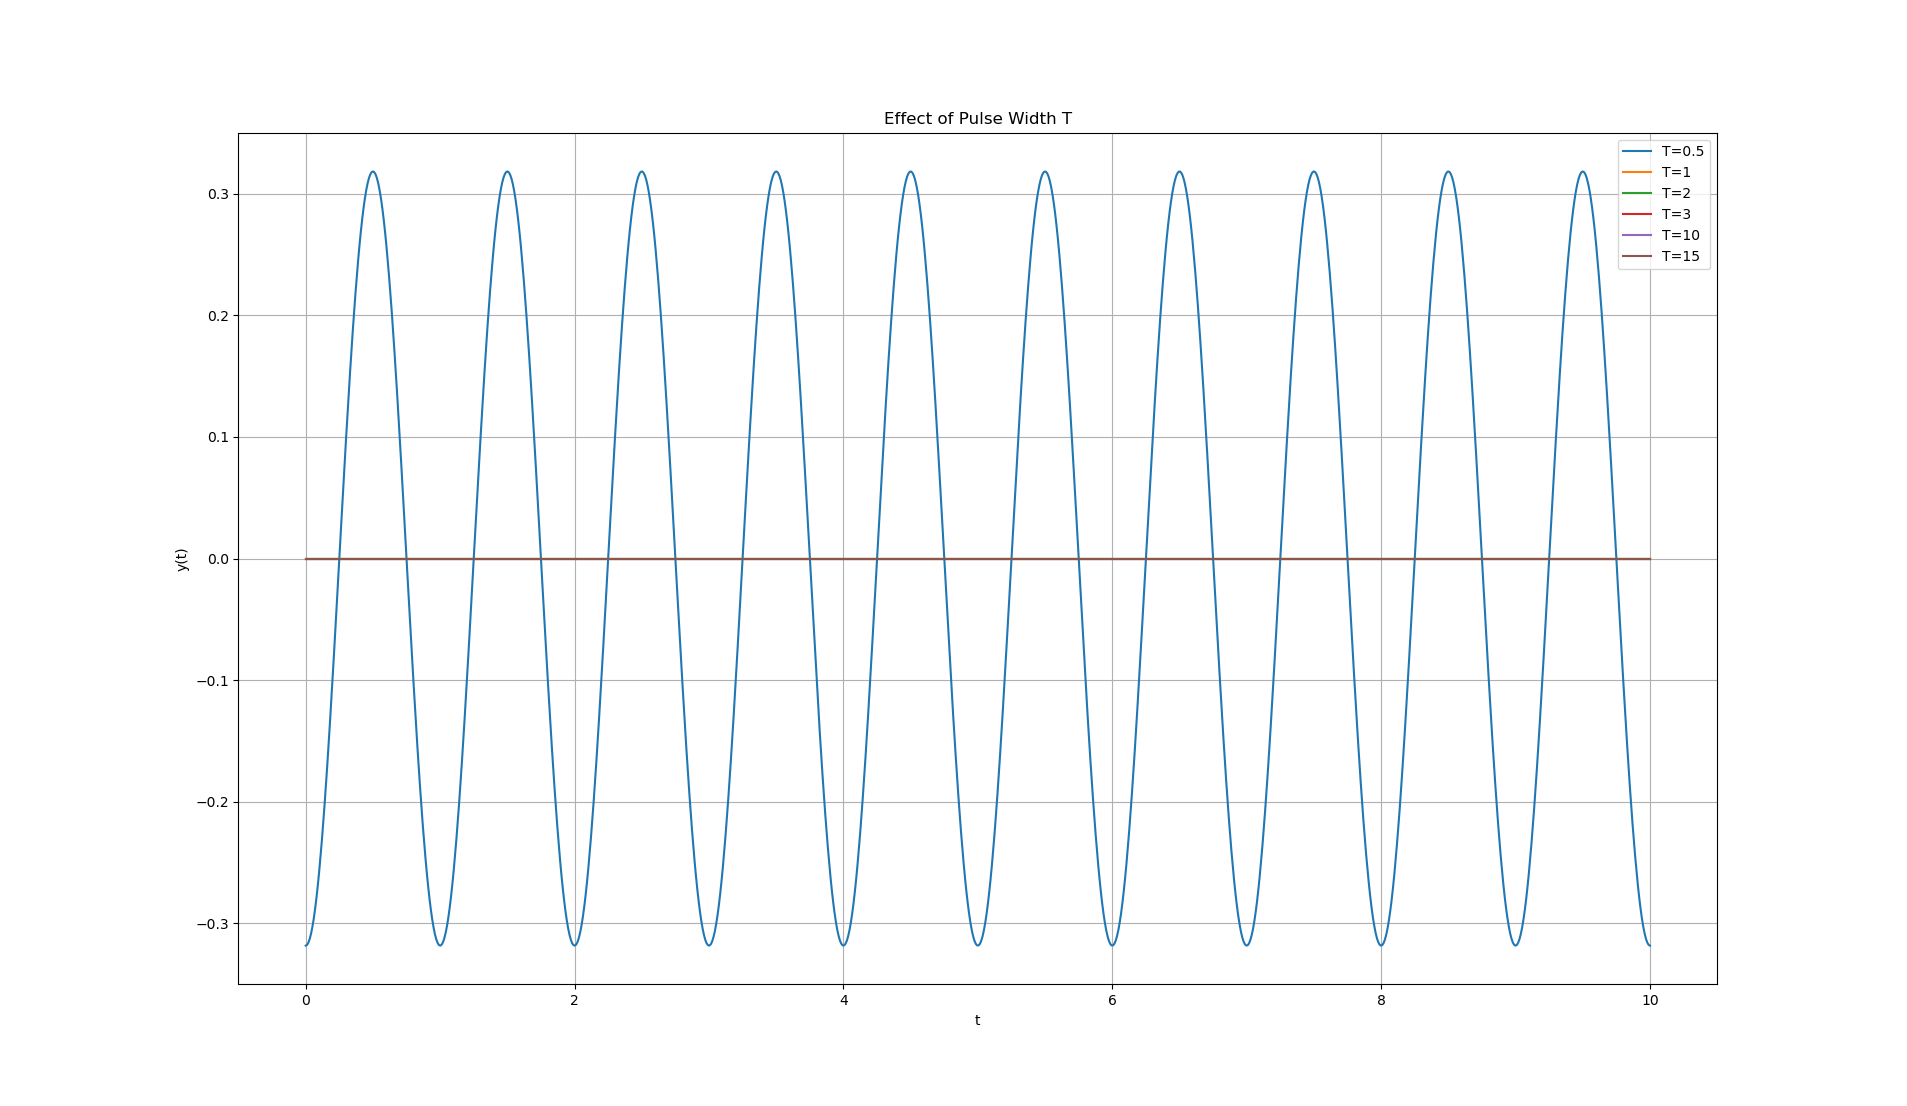
\includegraphics[width=0.8\textwidth]{codes/codes_sin_2/figs/T.png}
    \caption{Convolution output for different pulse widths \( T \).}
\end{figure}

\subsubsection{Amplitude Ratio vs Angular Frequency}

This plot captures the normalized amplitude ratio \( \frac{A_{out}}{A} = \frac{2\sin(\omega \frac{T}{2})}{\omega} \) as a function of \( \omega \) for various values of \( T \). It reflects the sinc-function behavior, emphasizing low-pass characteristics of convolution with rectangular kernels.
\begin{figure}[h]
    \centering
    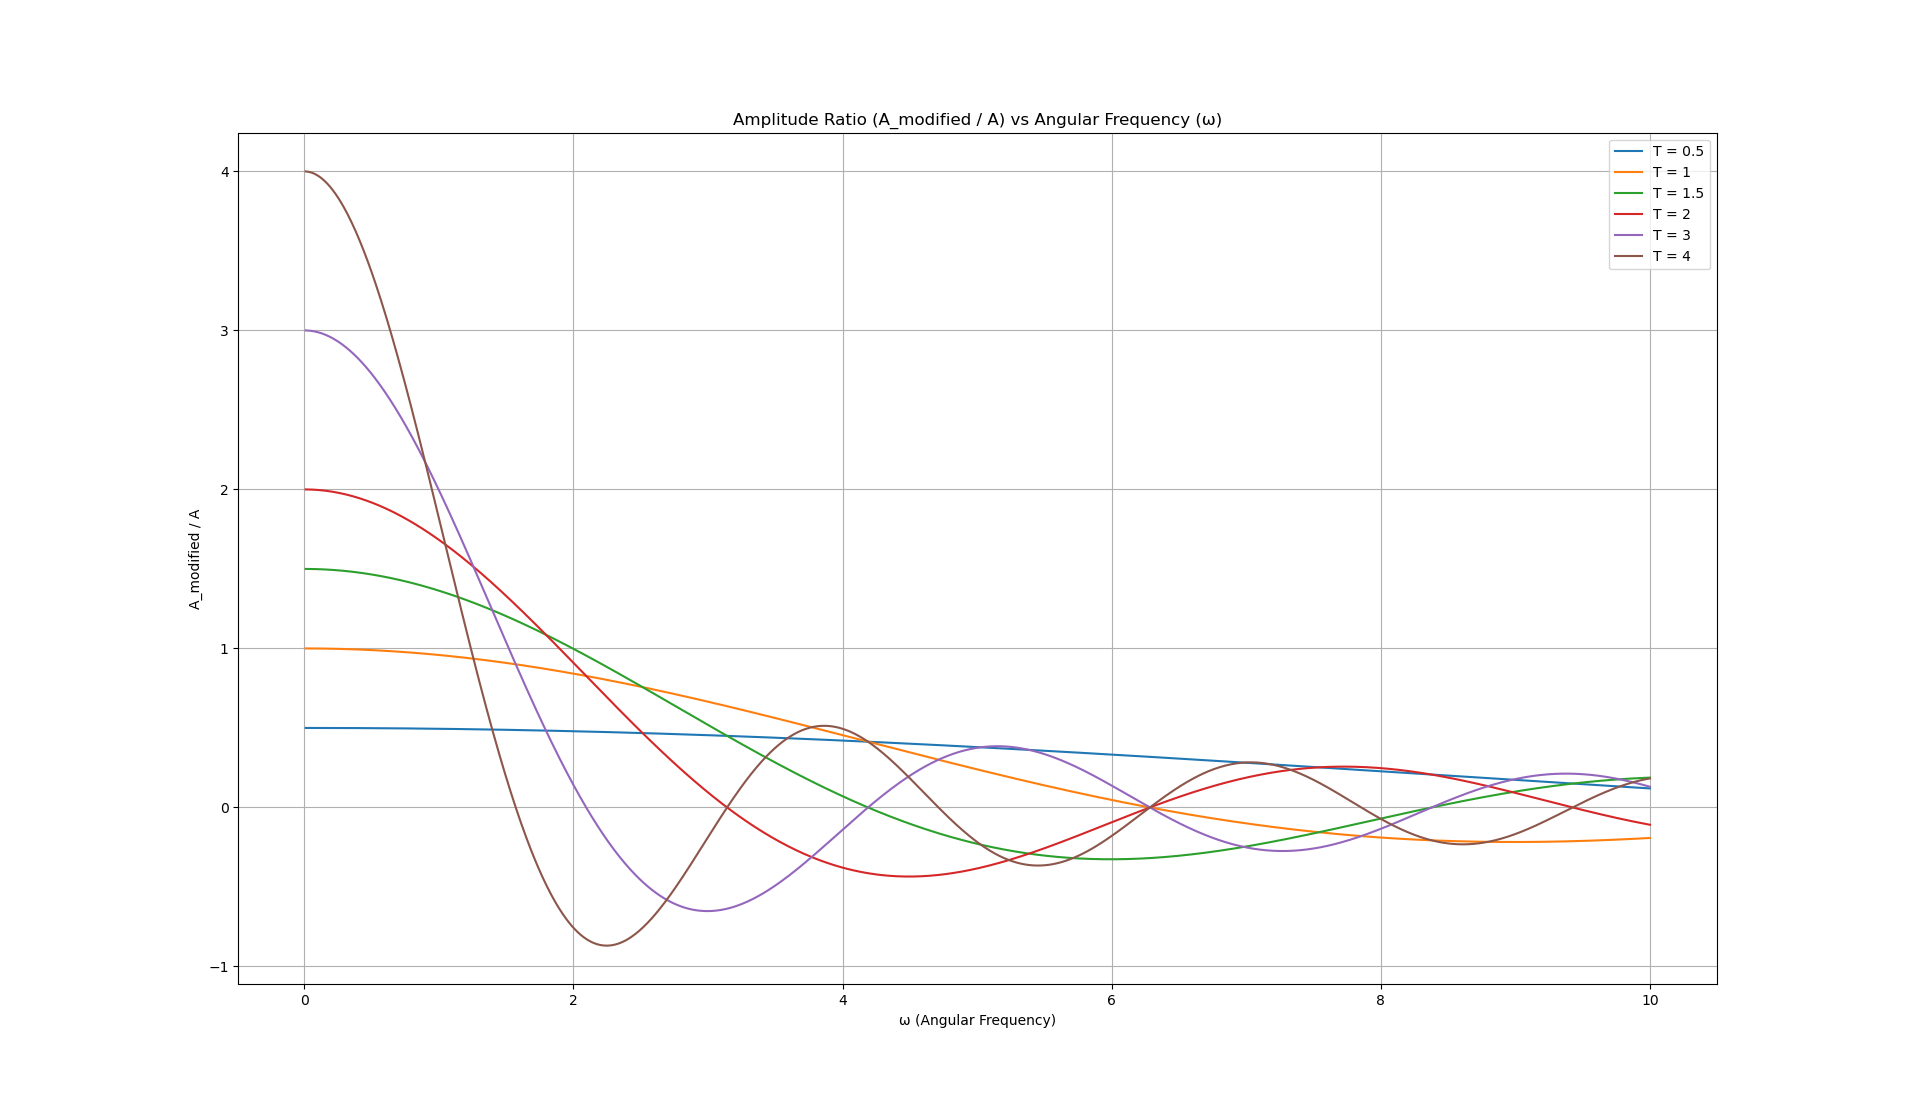
\includegraphics[width=0.8\textwidth]{codes/codes_sin_2/figs/scaling.png}
    \caption{Amplitude ratio \( \frac{A_{\text{modified}}}{A} \) versus angular frequency \( \omega \) for different values of \( T \).}
\end{figure}

\subsubsection{Effect of Phase \( \phi \)}

Altering the phase \( \phi \) of the sinusoidal signal results in horizontal shifts in the waveform. The output retains its shape but is delayed or advanced in time.
\begin{figure}[h]
    \centering
    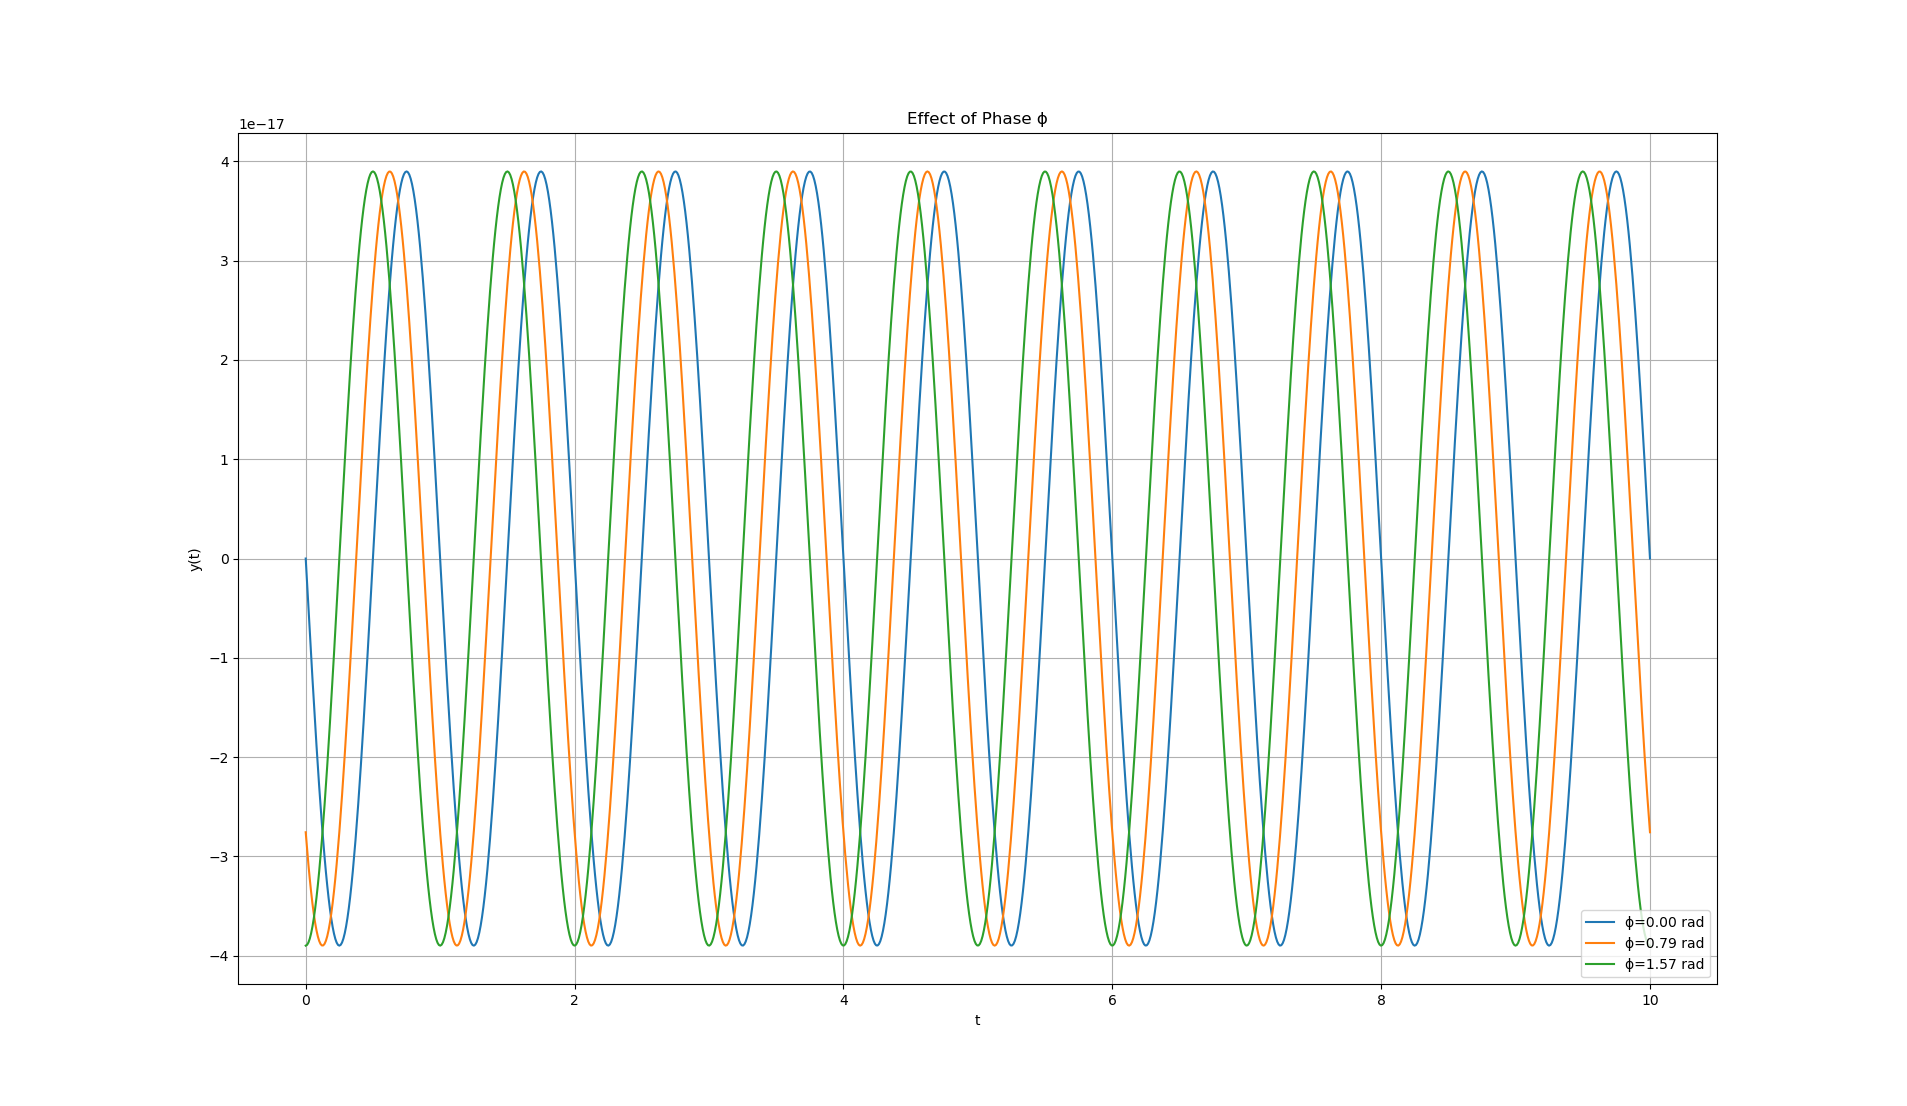
\includegraphics[width=0.8\textwidth]{codes/codes_sin_2/figs/phi.png}
    \caption{Phase shift \( \phi \) changes the horizontal alignment of the output signal.}
\end{figure}

\subsubsection{Special Observations}
\begin{itemize}
    \item If \( \omega T = n\pi \), the output vanishes, indicating frequency nulls.
    \item For large \( T \), the kernel acts as a low-pass filter.
    \item When \( T \rightarrow 0 \), the kernel approximates an impulse, and the convolution result tends to zero everywhere.
\end{itemize}

\subsection{Convolution with Varying Parameters}

The figure below shows the convolution output for multiple combinations of parameters including amplitude \( A \), frequency \( \omega \), kernel width \( T \), and phase \( \phi \). It highlights how these parameters influence the shape, scaling, and shift of the output signal.

Each sub-plot or curve within the figure corresponds to a unique configuration. You can observe:
\begin{itemize}
    \item Changes in amplitude due to scaling by \( \frac{2\sin(\omega T)}{\omega} \)
    \item Phase shifts resulting from both the signal phase \( \phi \) and kernel delay \( \tau_0 \)
    \item Smoothing effects due to increasing kernel width \( T \)
    \item Attenuation of high-frequency components, emphasizing the low-pass filter nature of box kernels
\end{itemize}

\begin{figure}[h]
    \centering
    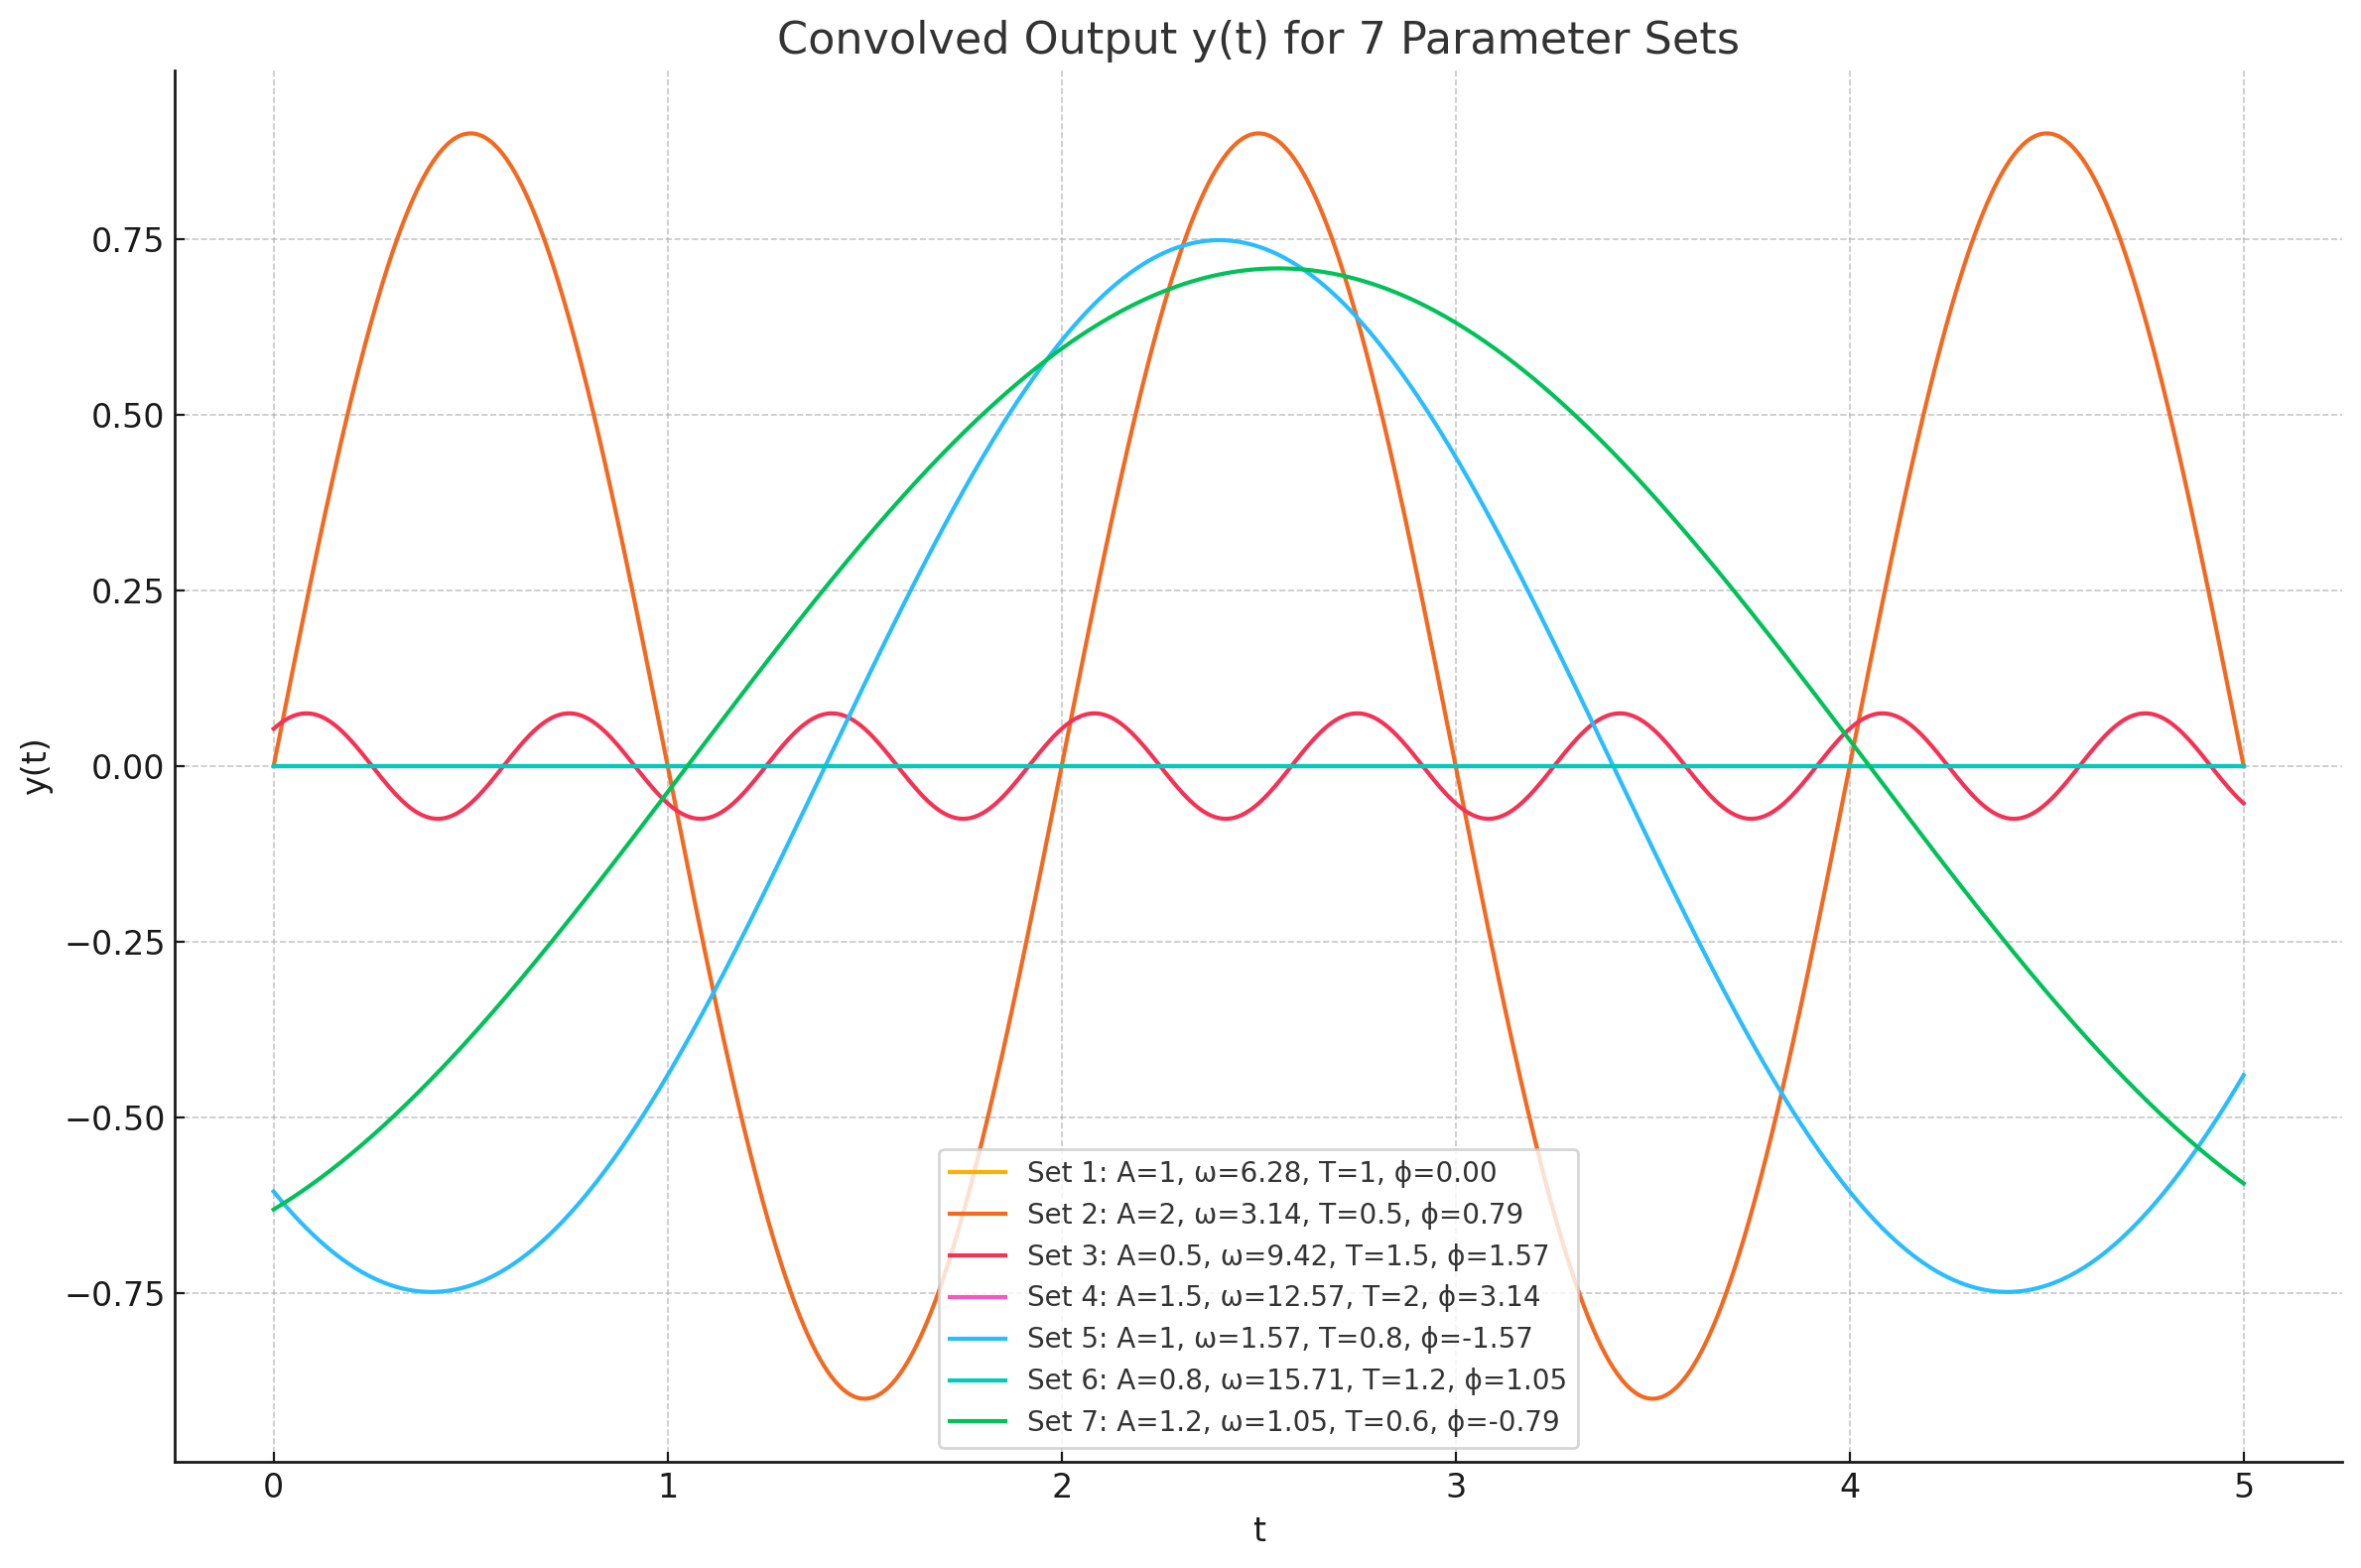
\includegraphics[width=0.7\textwidth]{codes/codes_sin_2/figs/all_varies.png}
    \caption{Convolution output for different parameter sets \( (A, \omega, T, \phi) \).}
\end{figure}


\subsection{Conclusion}

This detailed analysis of convolution using a rectangular kernel shows how parameters such as amplitude, frequency, kernel width, and phase influence the output signal. The kernel acts as a smoothing and low-pass filter, selectively attenuating high-frequency components. Additionally, time-shifting the kernel leads to equivalent shifts in the output, demonstrating important system properties like linearity and time invariance.

\end{document}
